\chapter{Procedure-Call comunication}
Prima lezione dopo i parziali.

\section{Remote Procedure Call}
Le procedure remote sono una estensione al distribuito del normale protocollo di chiamata di procedura.
\subsubsection{Vantaggi}
\begin{itemize}
    \item hanno una semantica nota: chiamata di procedura
    \item sono facili da implementare: vicine al modello client-server
\end{itemize}
\subsubsection{Svantaggi}
\begin{itemize}
    \item realizzate dal programmatore: tutto è esplicito [si può ovviare usando modelli a componenti più sofisticati]
    \item sono statiche: scritte nel codice dei programmi [si può ovviare usando chiamate indirette]
    \item non c'è concorrenza: sono bloccanti [si può ovviare con un uso appropriato dei thread o chiamate asincrone]
\end{itemize}

\section{Il modello RPC}
Il modello RPC maschera il modello client-server.
\begin{center}
    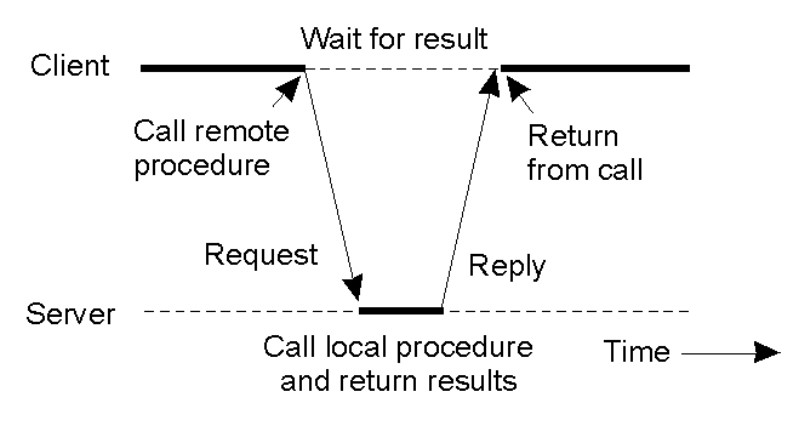
\includegraphics[scale=0.5]{img/RPC_modello1.jpg}
\end{center}
\subsection{Il modello RPC asincrono}
\begin{center}
    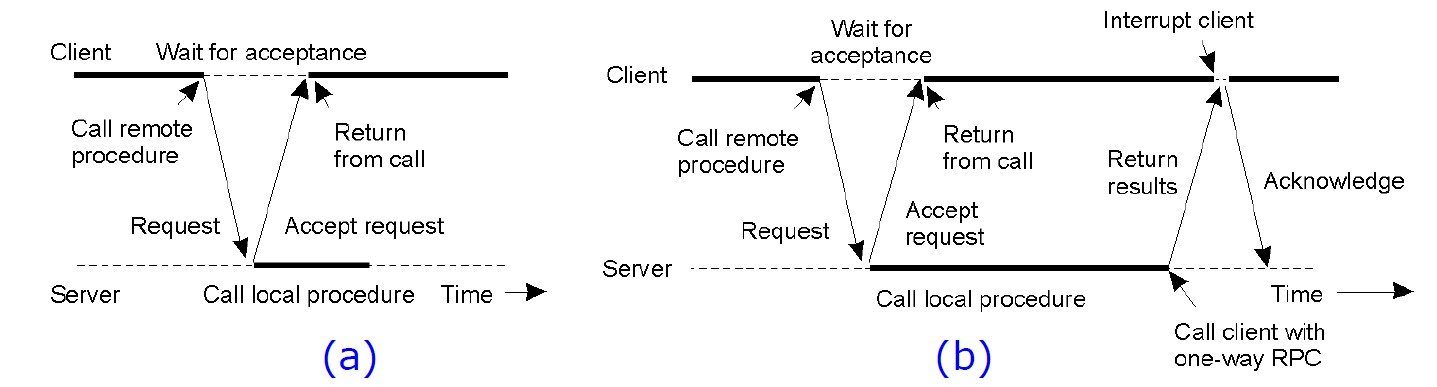
\includegraphics[scale=0.5]{img/RPC_modello2.jpg}
\end{center}
\begin{itemize}
    \item[] \textbf{a) \,} interazione tra client e server utilizzando una RPC asincrona, senza risposta
    \item[] \textbf{b) \,} interazione tra client e server utilizzando una RPC asincrona, con riposta posticipata utilizzando una seconda RPC asincrona (una call-back)
\end{itemize}
NOTA: poiché si realizza con scambio di messaggi, ricordare i modelli base studiati nella lezione «comunicazione a messaggi»

\section{Da PC a RPC}
\subsubsection{Lato client}
\begin{description}
    \item[Programma:] chi chiamare?
    \item[Middleware:] come interagire il programma cliente?
    \item[Middleware:] dove sta la macchina server?
    \item[Middleware:] come trattare i parametri?
\end{description}
\subsubsection{Lato server}
\begin{description}
    \item[Middleware:] quale procedura invocare?
    \item[Middleware:] come passare i parametri?
    \item[Middleware:] come trattare il risultato?
\end{description}

\section{Architettura RPC}
Si utilizzano degli stub per:
\begin{itemize}
    \item simulare comportamenti locali per chiamante e chiamato
    \item realizzare la comunicazione tra processi remoti
\end{itemize}
\begin{center}
    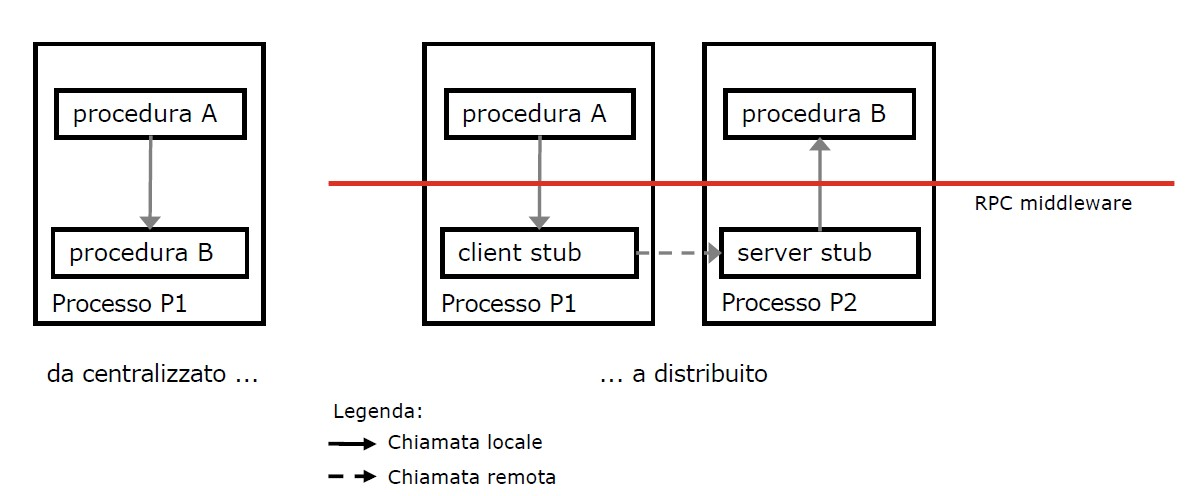
\includegraphics[scale=0.5]{img/RPC_architettura1.jpg}
\end{center}

\section{Passing Value Parameters}
Steps involved in doing remote computation through RPC.
\begin{center}
    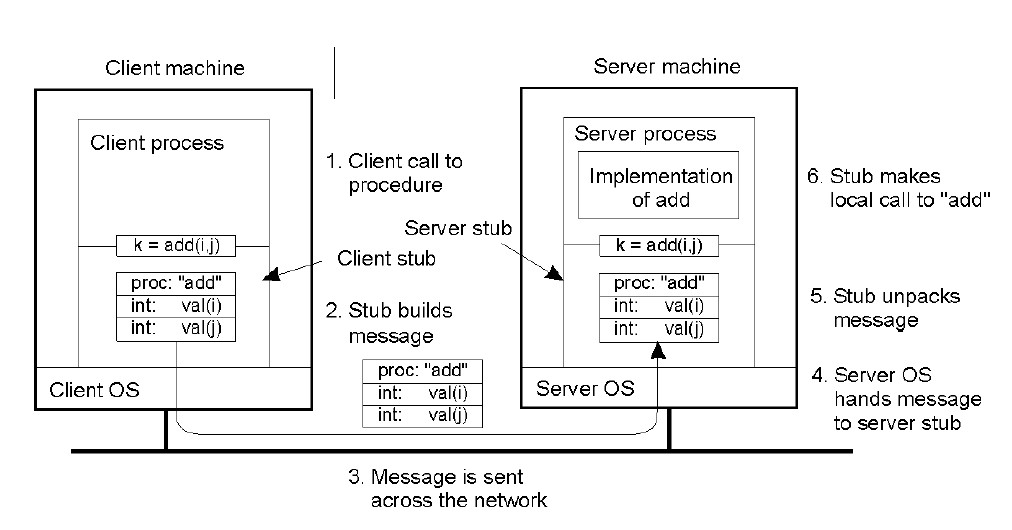
\includegraphics[scale=0.5]{img/RPC_passaggioparametri1.jpg}
\end{center}

\subsection{Passaggio parametri Procedure Call locale}
I parametri sono passati per: puntatore, valore.
\\Esempio: prodotto tra matrici.
\begin{verbatim}
    1. void main() {
    2.   Matrix A, B, C;
    3.   int size = ...;
    4.     ...
    5.     C = call mtxmpy(A, B, size);
    6.     ...
    7. }
\end{verbatim}
\begin{center}
    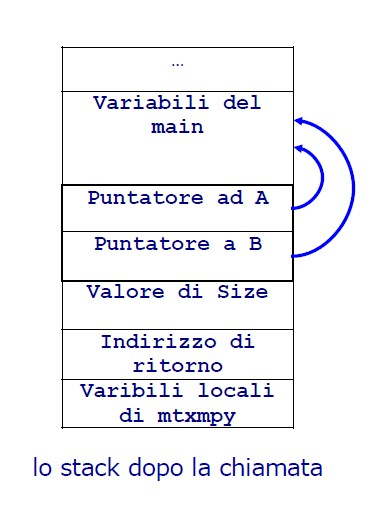
\includegraphics[scale=0.5]{img/RPC_passaggioparametri2.jpg}
\end{center}

\subsection{Passaggio parametri Procedure Call remota}
Replica dello stack nel processo remoto: i dati vengono "impacchettati", spediti, "spacchettati" per creare copie locali.
\\L'operazione si chiama marshalling/unmarshalling dei dati.
\begin{center}
    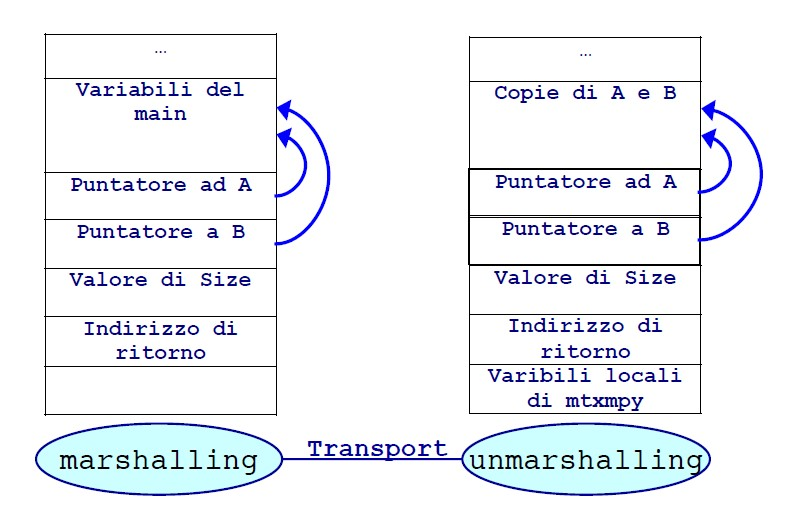
\includegraphics[scale=0.5]{img/RPC_passaggioparametri3.jpg}
\end{center}

\section{Esecuzione di una RPC}
\begin{center}
    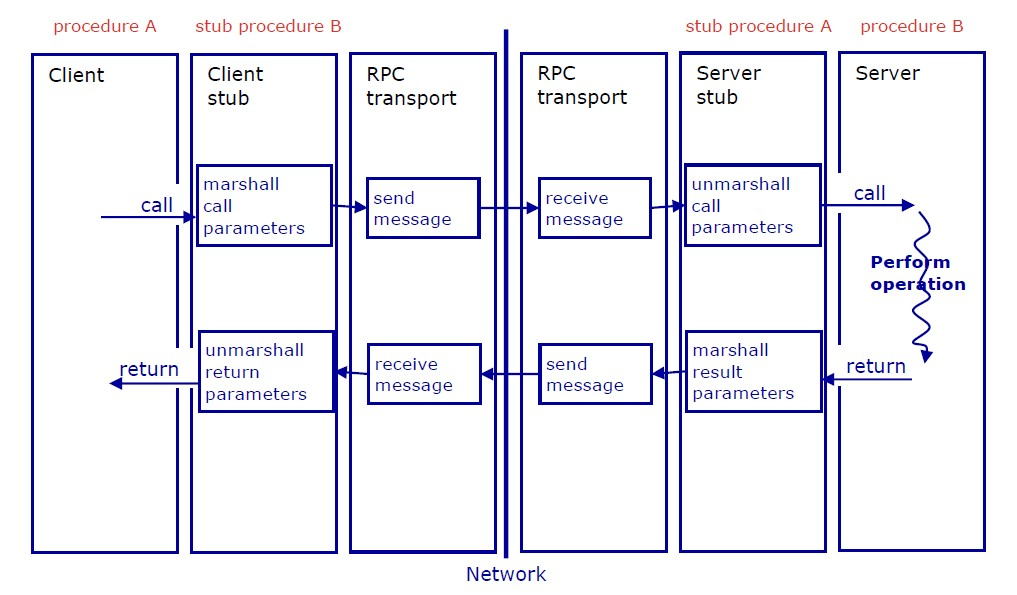
\includegraphics[scale=0.5]{img/RPC_esecuzione1.jpg}
\end{center}

\chapter{Oggetti Distribuiti}
Architettura di riferimento:
\begin{center}
    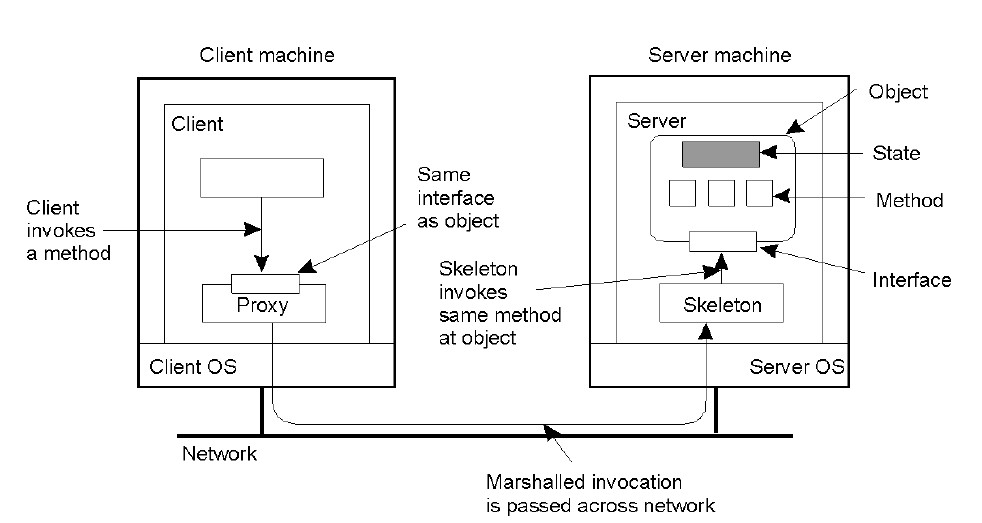
\includegraphics[scale=0.5]{img/DO_architettura1.jpg}
\end{center}
\section{Caratteristiche}
\subsubsection{Oggetti}
\begin{itemize}
    \item Incapsulano i dati (stato) - I valori dei campi o variabili
    \item Definiscono operazioni sui dati - I metodi delle classi
    \item Definiscono l'accesso - I metodi delle interfacce
\end{itemize}
\subsubsection{Oggetti a compile-time}
\begin{itemize}
    \item Definiti attraverso interfacce e classi (Java, C++)
\end{itemize}
\subsubsection{Oggetti a run-time}
\begin{itemize}
    \item Accessibili attraverso adapters (wrappers)
\end{itemize}
\subsubsection{Oggetti persistenti e transienti}
\subsubsection{Riferimento agli oggetti remoti}

\section{Pointers vs. references}
Differenze fra puntatori e riferimenti in C++:
\begin{center}
    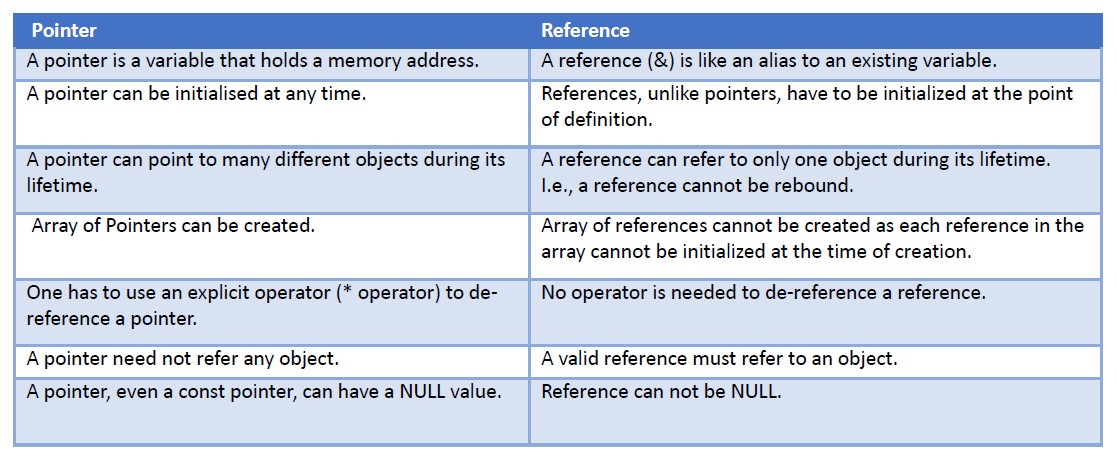
\includegraphics[scale=0.5]{img/DO_pointersreferences1.jpg}
\end{center}
\subsubsection{Un puntatore (pointer in C/C++)}
\begin{itemize}
    \item è una variabile che contiene un indirizzo di memoria (che può contenere qualsiasi cosa)
    \item può essere modificato in ogni momento -> aritmetica dei puntatori
    \item non è tipizzato (può riferirsi ad un oggetto o ad altro)
\end{itemize}
Un \textbf{puntatore distribuito}
\begin{itemize}
    \item non può esistere (non avrebbe senso)
\end{itemize}
\subsubsection{Un riferimento (reference in Java)}
\begin{itemize}
    \item è una variabile che contiene informazioni logiche (alias) per accedere ad un oggetto
    \item è immutabile -> può essere inizializzato all'atto della creazione di un oggetto
    \item è strongly typed -> la classe dell'oggetto definisce il tipo
\end{itemize}
Un \textbf{reference distribuito}
\begin{itemize}
    \item Indirizzo della macchina
    \item Indirizzo (porta) del server (processo)
    \item Identificatore (ID) dell'oggetto
\end{itemize}

\section{Passaggio di parametri}
Passaggio parametri per reference o per valore.
\begin{center}
    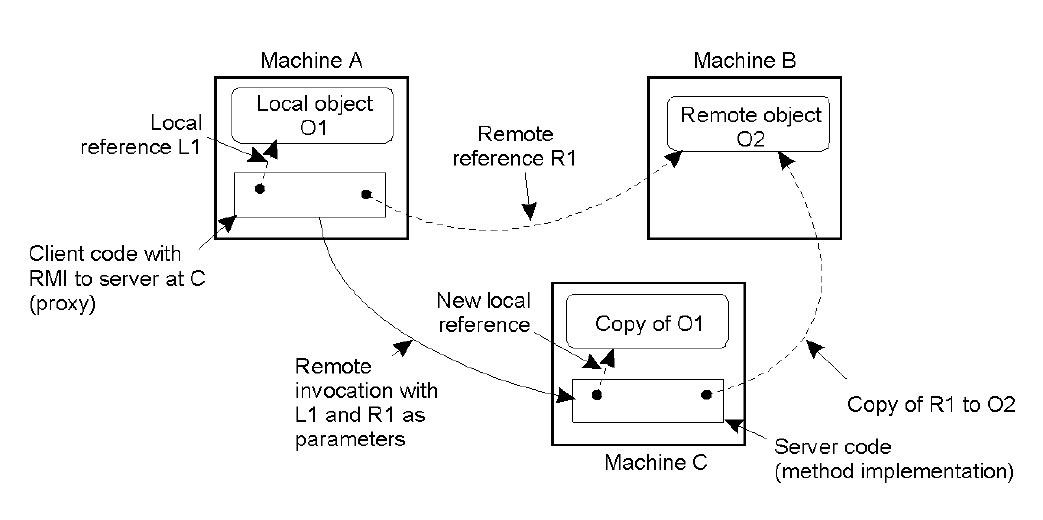
\includegraphics[scale=0.5]{img/DO_passaggioparametri1.jpg}
\end{center}
Locale: più relativo. Remoto: più assoluto.

\chapter{Java RMI (Remote Method Invocation)}
\section{Il middleware RMI}
RMI è un middleware che:
\begin{itemize}
    \item estende l'approccio OO al distribuito: supporta l'inheritance
    \item supporta l'invocazione di metodi tra oggetti su macchine virtuali distinte
    \begin{itemize}
        \item le interfacce sono Java (non in un IDL generico)
        \item vengono passati e ritornati oggetti Java
        \item le classi vengono caricate dinamicamente
    \end{itemize}
    \item si basa sulla portabilità del bytecode e sulla macchina virtuale: più sicuro (safe) ed efficiente perché non si deve tradurre nulla
    \item fornisce servizi:
    \begin{itemize}
        \item caricamento e controllo con un class loader e un security manager
        \\• https://docs.oracle.com/javase/8/docs/api/java/lang/ClassLoader.html
        \\• https://docs.oracle.com/javase/tutorial/essential/environment/security.html
        \item gestione di oggetti remoti, replicati, persistenti
        \item attivazione automatica degli oggetti
        \item multi threading
        \item garbage collection di oggetti remoti con un meccanismo di conteggio dei reference
    \end{itemize}
\end{itemize}

\section{The Java Environment}
\begin{center}
    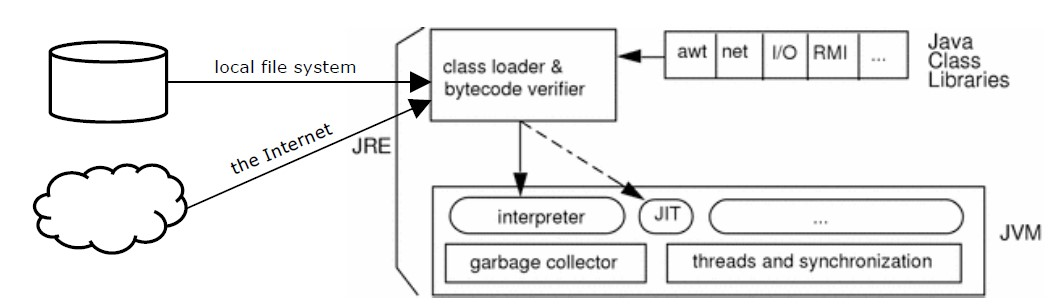
\includegraphics[scale=0.5]{img/RMI_JE1.jpg}
\end{center}
The class loader is in charge of loading classes • The bytecode format allows the loader to transfer .class files either from libraries, local file systems, or network domains.
\\The loading activity occurs dynamically when 
\begin{itemize}
    \item a "new" command is performed, or
    \item a RMI object is transferred
\end{itemize}
https://docs.oracle.com/cd/E19455-01/806-3461/6jck06gqb/index.html
\\https://docs.oracle.com/javase/tutorial/ext/basics/load.html

\subsection{Invocazioni}
JavaRMI - Remote Method Invocation
\begin{itemize}
    \item Simile a RPC per la gestione parametri per valore
    \item Consente anche passaggio parametri per reference
    \item Definisce stub specifici per ogni oggetto (in RPC sono generici)
\end{itemize}
Invocazioni statiche
\begin{itemize}
    \item Interfaccia nota in compilazione
\end{itemize}
Invocazioni dinamiche
\begin{itemize}
    \item L'invocazione include informazioni logiche sull'identita' dell'oggetto e del metodo
    \item Invoke(obj, method, input_parameters, output_parameters)
    \item (argomento non trattato per mancanza di tempo)
\end{itemize}
